\documentclass[11pt, a4paper, notitlepage]{report}
\usepackage[round,colon]{natbib}
\bibliographystyle{hull}
\usepackage[utf8]{inputenc} % Ensures we can use UTF8.
\usepackage{pdflscape}
\usepackage{graphicx}
\usepackage{hyperref} % Must come last; allows for links.
\hypersetup{
    hidelinks
}
% Details.
\title{Smart Kart (Project Initiation Document)}
\date{November 2021}
\author{George Jacob Anthony Kokinis}

\begin{document}

\maketitle
\begin{center}
    Student Number 201910280
    
    Word Count: 2054 %exclude acknowledgements, abstract, table of contents, references and appendices) of your document.
\end{center}
\newpage

\tableofcontents

\chapter{Project Background and Purpose}
\section{Objectives}
This project seeks to create a software application for a smartphone, that 
detects when a vehicle the phone is in enters an "Average Speed Check zone", 
starts tracking the vehicle's speed, and gives the driver an audible alert if 
they are at risk of breaking the speed limit.

The usefulness of this project is the safety benefits it may provide. If the 
application produced can reduce the frequency that a driver needs to check 
their speedometer, then they will be more aware of road conditions; which can 
lead to safer driving.

This project is motivated by the increasing deployment of average speed check 
zones throughout the UK (doubling between 2013 and 2016 
\citep{BBCSpeedCameraDoubled}), and the potential they may have for leading to 
distracted driving.

\subsection{Primary Objectives}\label{subsec:PrimaryObjectives}
The Primary Objectives of this project are:
\begin{itemize}
    \item To develop an app (for a smartphone) that determines when the user is 
    in an "average speed check zone", and begins tracking average speed.
    \item Said app then warns, with an audible warning, if the user's average 
    speed is above the limit.
    \item Voice commands may be used to launch the app at the user's request 
    (for example, if there is temporary speed check area).
\end{itemize}

\subsection{Secondary Objectives}
If time allows, the project may achieve the following objectives:
\begin{itemize}
    \item The app allows for the user to manually set what the speed limit is 
    (for example if a road has a temporarily reduced speed limit).
    \item The app allows for setting the audible warning to a custom sound.
\end{itemize}

\subsection{Tertiary Objectives}
In many territories globally, the use of devices to detect speed cameras is 
illegal, and apps are either explicitly or potentially illegal; for example in 
France, any device or system used to "detect the presence" of devices for 
regulation of road traffic, is illegal under the Code de la route 
\citep{CodeDeLaRoute}.
It would be ideal if the app could detect it was in such a territory, and 
prevent its own usage.

As well, the app may allow the users to contribute to an open dataset of 
average speed check zones.

\section{Scope}\label{sec:Scope}
There is scope within the project to provide an app that is cross platform, 
using technologies such as Flutter, UNO, and .NET MAUI (née 
Xamarin.Forms)\footnote{Flutter \citep{FlutterWebsite}, UNO \citep{UnoWebsite}, 
.NET MAUI \citep{UnoWebsite}}. This would allow users of the major mobile 
ecosystems to use the app. 

However, doing so requires a developer to be familiar with the relevant tooling 
and languages (Dart for Flutter, C\textsubscript{\#} for UNO and MAUI). If a 
developer is not familiar, learning the tooling may take up a significant 
amount of time that should be spent on the actual programming. Hence, we are 
presented with a choice to be made during the analysis stage of the project.

There is also scope to build an independent database of average speed check 
areas; this would bring "server-side" programming into the project. 
Alternatively, there may already be public datasets available for use. Whether 
to use existing datasets (if possible) or build an independent one is another 
decision for the analysis stage. 

Should the project opt to use public dataset(s), allowing for contribution to 
such datasets from within the app would serve the public good and benefit the 
app's users; so this may well be within the scope of the project.
% include example datasets?

\section{Deliverables}
The Project will deliver a smartphone application that meets the Primary 
Objectives (defined in section \ref{subsec:PrimaryObjectives}).

The project will have met its objectives when the app matches provides features 
defined by the Primary Objectives. If the project \textbf{also} implements 
Secondary or Tertiary Objectives, it may be considered to have "exceeded" its 
objectives.

\section{Constraints}\label{sec:Constraints}
Testing the application in the most \textit{direct} way - using the app while 
driving - may be constrained by:
\begin{itemize}
    \item Law: It's illegal to use a mobile phone whilst driving, under the 
    Road Vehicles (Construction and Use) Regulations, 1986 (amended 2003):110 
    \citep{RoadVehiclesSI}.
    \item Insurance: most motor insurers aren't favourable to claimants using 
	their mobile phones. Furthermore, most insurance doesn't cover "testing" on 
	public nor private roads.
    \item Ethics: The University of Hull's Research Ethics Policy 
    \citep{HullEthicsPolicy} defines "non-malfeasance" as the "avoidance of 
    harm". Testing the application in the above way flies in the face of this, 
    as driving distracted is an easy way to cause harm.
\end{itemize}
The obstruction this causes to testing can be mitigated through the use of an 
emulated device and "falsified" location data.

Otherwise, there are no external constraints known at this time.

\section{Assumptions}
There are currently no unknowns for this project; hence, there are no 
assumptions to be made.

\chapter{Project Rationale and Operation}
\section{Project Benefits}
Successful delivery of this project will most benefit car drivers (primarily in 
the UK, but possibly in other territories), with phones, who often drive in 
areas with average speed check zones. 

By reducing the time spent monitoring their speedometer, they can be more 
conscious of the road around them, and be more alert to potential incidents.

As well, by providing \textit{advance} warning of exceeding the average speed, 
they may be able to drive in a smoother manner and avoid the "kangaroo-ing" 
effect, as seen when a driver brakes harshly to avoid a ticket; this can reduce 
congestion and prevent accidents.

\section{Project Operation}\label{sec:projectOperation}
Agile Software Development is a paradigm, commonly defined by the Manifesto \citep{AgileManifesto}; within this paradigm are many varied methodologies. For 
projects where there is only one team member, methodologies such as Kanban and 
Scrum (as modified by Scrum for One \citep{ScrumForOne}) are optimal. %% FInd a source on this!!

The Kanban board is a useful tool to understand the current state of the 
project; what is in progress, what needs to be started, etc. Combined with the 
user-input and cyclical nature of the Agile paradigm, this is ideal for a 
project like this one, with one developer and fast development times.

The overall planning and schedule for this project is laid out in the Gantt 
Chart in section \ref{subsec:schedGanttCt}. The intention is to stick with this 
schedule; however, the agile paradigm requires flexibility, so this may change 
with time.

\section{Options}
As discussed in the section on Scope (\ref{sec:Scope}), for developing this 
project there is certainly one choice to be made: is the app developed using 
one of various cross-platform frameworks, or using platform-native frameworks.

While it was not decided in that discussion whether to use cross-platform or platform native, there are choices within platform-native that are pertinent to discuss here.

\subsection{Which Platform?}
The Project's nature requires a mobile platform. However, there is a choice 
within this; despite Android and iOS' apparent dominance of the market (with 
\citet{MobileMarketShare} claiming combined a 99.19\% share, as of September 2021), there are various other mobile platforms, such as Tizen\footnote{Backed by the Linux Foundation, but primarily developed by Samsung.}, KaiOS, and Sailfish OS; as well as mobile implementations of desktop platforms, such as pureOS.

Despite this variety, Android stands tall as the easiest to develop for and 
most accessible platform. The Android Open Source Project means that obtaining 
an image to test on, or examining the OS' source to aid in debugging, is 
relatively easy. Hence, should platform-native be chosen, Android is an ideal platform to develop this project for. Furthermore, using Android Jetpack\footnote{Android Jetpack \citep{AndroidJetpack}} whenever possible will provide the project with a consistent base to build upon.

In comparison, developing platform-native applications for iOS devices requires 
a MacOSX device (real or emulated, either of which are expensive) to use Xcode, and a payment of \$99 if you wish to distribute your application on the Apple App Store \citep{AppleDevProgram}. This is significant outlay for a small development team. The other mobile platforms have significantly small market share.

\subsection{Which Language?}
Android applications have historically been written in Java, and the foundation 
of the OS is a JVM (originally Dalvik but later ART). The ecosystem around Java 
on Android is mature and well-documented.

However, in 2011 JetBrains\texttrademark\ announced Kotlin, a JVM language 
"having the features so desperately wanted by the developers" \citep{KotlinAnnounced}. Being a JVM language, it was inherently "usable" on Android; but the Android Team announced "first-class support" in 2017 \citep{KotlinPreferred} and "Android development will become increasingly Kotlin-first," in 2019 \citep{KotlinFirst}.

Hence, this project could develop the app in Kotlin or in Java. Kotlin is now 
the contemporary language, and Google suggests that "If you’re starting a new 
project, you should write it in Kotlin" \citep{KotlinFirst}; however, Java already has a massive ecosystem surrounding it.

\section{Risk Analysis}
The most major risks to the Project at this time are those associated with 
Covid-19: Potential future lockdowns, mutations of the virus, supply issues, 
and potential infection of the Author. These risks can be mitigated by the 
actions of the Author, but only to an extent; it depends upon the actions of 
others as well.

There are various other risks, such as personal illness, strikes, and equipment 
breakdowns; the analysis table is in Appendix \ref{app:RiskAnalysis}.

\section{Resources Required}
There are no abnormal resources required for this project. All that is needed 
is a computer to develop on, and an android phone (or the AVD emulator) to test 
with.

If any of these were unavailable (for example, if the computer being used 
became non-functional), it would delay the project until an alternative could 
be sourced, or until the University's Labs are available.
%What resources will you need for the project?  Are any non-standard?  Are they 
%already available?  What effect will it have if they are not available or are 
%delayed, and how would you manage that?

\chapter{Project Methodology and Outcomes}
\section{Initial Project Plan}
\subsection{Tasks and Milestones}
%Present a realistic task list for the entire project, broken down to a 
%suitable level of detail.  Indicate milestones against which progress can be 
%monitored.
The tasks for developing the application can be broken down into Milestones. 
Within milestones, tasks may be performed asynchronously and simultaneously; 
but generally, milestones are dependant on the previous milestone.

\begin{enumerate}
    \item [Milestone 1:]Design and Architecture.
    \begin{itemize}
        \item Evaluate potential application designs and architectures.
        \item Plan the overall application architecture.
    \end{itemize}
    \item [Milestone 2:]UI and UX.
    \begin{itemize}
        \item Plan the User Interface (UI) design.
        \item Plan the User Experience (UX).
        \item Implement the UI.
        \item Implement the UX.
        \item Testing of the UI and UX.
    \end{itemize}
    \item [Milestone 3:]Average Speed Algorithm.
    \begin{itemize}
        \item Evaluation of Algorithms for determining average speed.
        \item Implementation of Algorithm.
        \item Algorithm Testing.
    \end{itemize}
    \item [Milestone 4:]Determining if the Device is within an Average Speed Check Zone.
    \begin{itemize}
        \item Evaluation of potential Datasets.
        \item Design of Data Model.
        \item Implementation of Data Model.
    \end{itemize}
    \item [Milestone 5:]Glue Code, Bug Fixes, Further Objectives, and Delivery.
    \begin{itemize}
        \item Creation of any "glue code" necessary; for example, changes to 
        build tools, code necessary to publish on the Play Store/F-Droid, etc.
        \item Bug fixes: Any final bug fixes for issues not found during 
        testing in prior milestones.
        \item If time permits, Secondary and Tertiary Objectives will be 
        delivered under this milestone.
        \item Delivery of the final Artefact.
    \end{itemize}

Alongside these tasks, there is the singular long-running task of writing the 
final report.
\end{enumerate}
\subsection{Schedule Gantt Chart}\label{subsec:schedGanttCt}
The Gantt chart here is not as detailed as the task list above. This is due to 
the project using Agile and Kanban, meaning that tasks can be running 
out-of-order, simultaneously, and asynchronously; which isn't easily 
represented on a Gantt chart. Hence, the chart is more of a "timeline", and 
this PID also includes a snapshot of the initial state of the Kanban board, 
found in appendix \ref{app:KanBan}. This initial state may change upon 
commencement of the report and the creation of User Stories, Epics, etc.
\begin{landscape}
    \begin{figure}[h]
        \makebox[\textwidth][c]{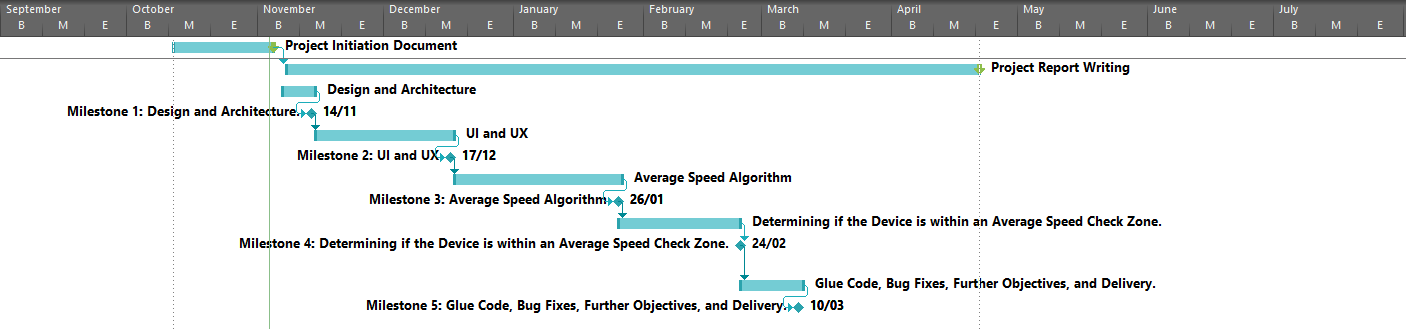
\includegraphics[width=1.3\paperwidth]{GanttChart.png}}
        \centering
        \caption{Gantt Chart at the time of the PID.}
        \label{fig:ganttchart}
    \end{figure}
\end{landscape}
%Present a Gantt chart showing a schedule for all tasks, milestones and 
%deliverables. Show dependencies amongst tasks.

\section{Project Control}
Management of the project will be through the use of the Kanban board. The 
start of any development session begins by inspecting the board to understand 
the state of play. Then, the developer shall choose a task that is already in 
development (or if there are none, a task that hasn't been started), and work 
on it for the session.

Performance will be monitored based on the rate of progress through tasks. 
Should tasks take too long to complete, this is an indicator of a low 
performance. However, the inverse, tasks being completed quickly, is not 
inherently an indicator of high performance; it may well mean that tasks are 
not being completed to sufficient depth.

Whether the project is successful will be judged based on the resulting 
artefact, and whether this artefact has met the objectives in 
\ref{subsec:PrimaryObjectives}.

\section{Project Evaluation}
Evaluation of the Project's artefact(s) will be based on how close it adheres 
to the objectives in \ref{sec:projectOperation}.

In terms of User Evaluation, testing the entire application is limited by the 
constraints layed out in \ref{sec:Constraints}. However, the UI/UX could 
possibly be tested by users, independent of the underlying application.

\appendix
\chapter{Initial Kanban Board}\label{app:KanBan}
\begin{figure}[h]
    \makebox[\textwidth][c]{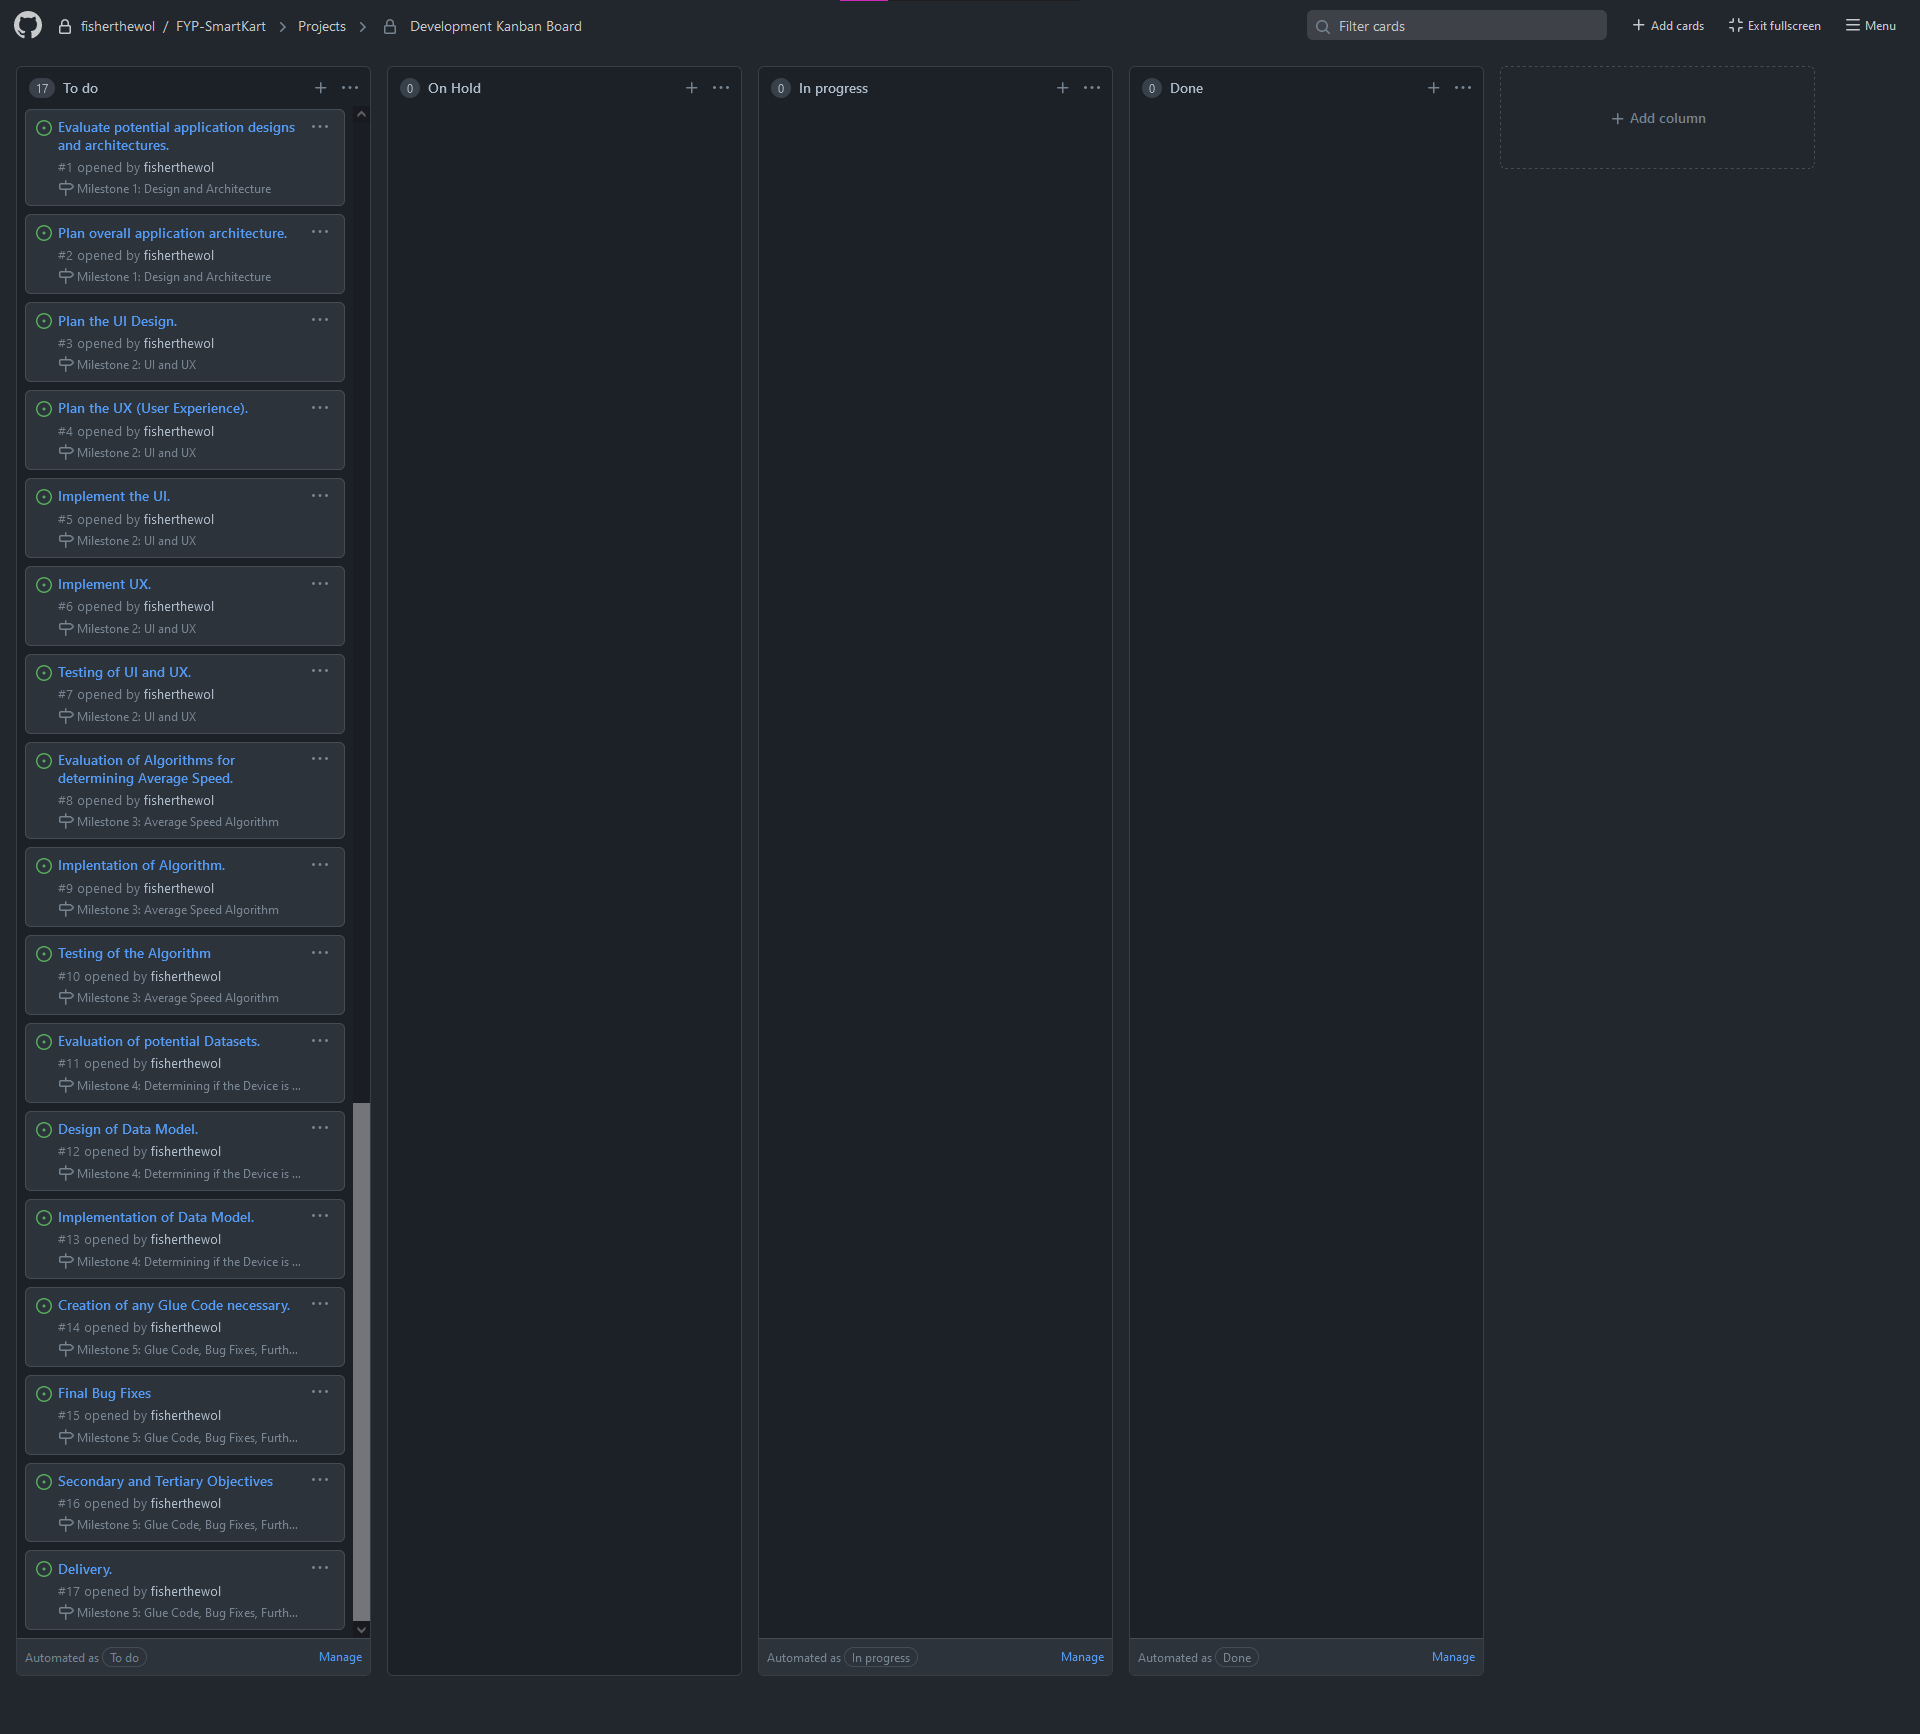
\includegraphics[width=0.7\paperwidth]{KanbanBoardMerged}}
    \centering
    \caption{Initial state of the Kanban Board.}
    \label{fig:kanbanboardmerged}
\end{figure}

\chapter{Risk Analysis Table}\label{app:RiskAnalysis}
\begin{table}
    \begin{tabular}{p{0.3\textwidth} p{0.5\textwidth} c c c p{0.5\textwidth} p{0.5\textwidth}}
        Risk &
        Description &
        Likelihood &
        Severity &
        Impact Score &
        Mitigation Taken &
        Recovery \\
        Total Equipment Failure &
        The Author's equipment (computer, phone) experiences total failure, preventing progress on the project until repaired. &
        1 &
        4 &
        4 &
        Regular Maintenance is performed on the equipment, and backups are made. As well, the data for this Project is stored as a repository on Github, so data loss should be minimal. &
        The Author shall use the University of Hull's library computers, until such a time as replacement equipment can be sourced. \\
        Partial Equipment Failure &
        A part of the Author's equipment fails, degrading the ability to progress with the project. &
        1 &
        3 &
        3 &
        Very similar to Total Equipment Failure, mitigation relies on maintenance, backup, and Github. &
        Similar to Total Failure, Hull University's library has computers available for student use. \\
        Covid Lockdown &
        The UK goes into another lockdown due to rising covid cases, preventing access to campus and &
        2 &
        3 &
        6 &
        Covid is a public health issue, hence mitigation requires societal collaboration on individual actions, such as mask wearing and social distancing. &
        Lockdown won't directly affect the writing of code in this project, but may affect the Author's mental health, or other health aspects. Hence, recovery involves mental wellbeing and awaiting the end of lockdown. \\
        Use of Phone in a Car &
        While testing the application, bugs or other issues cause distracted driving, which leads to a vehicular accident, injury, or death. &
        1 &
        4 &
        4 &
        The app will not be tested on the public roads. Instead it will be tested using the Android Emulator. &
        There is no recovery from death. However recovery from Injury involves various medical treatments. \\
        Application causes Damage to a device. &
        The application, through serious errors, causes physical or "software"" damage to a user's device." &
        1 &
        4 &
        4 &
        The app will not use obscure and undocumented features of the platform, unless absolutely necessary. This shifts the risk from the application to the developers of the standard library of the platform. &
        A device damaged by the application would be sent to a repair shop/manufacturer for repair. \\
        Application gives user false average speed. &
        The application either miscalculates the average speed of the vehicle, or believes the speed limit is higher than it actually is; leading to the user speeding and receiving a fine. &
        2 &
        2 &
        4 &
        Regarding the miscalculation: comprehensive software tests and a thorough review and understanding of the relevant kinematics will reduce the chance of miscalculation. Regarding the erroneous speed limit: this is mitigated by allowing the user to set their own speed limit outside of what is automatically detected, and by attempting to keep the dataset in use up to date. &
        There is not much the application can do to recover the speeding fine the user may receive; however, reports of such issues should be used as feedback to improve the application.
    \end{tabular}
\end{table}

\bibliography{pidbib}
\end{document}
